\section{Additional Experiments}\label{sec:additional-results}

In this section we present additional and extended results from the main section.

\begin{figure}[hbpt]
  \centering
  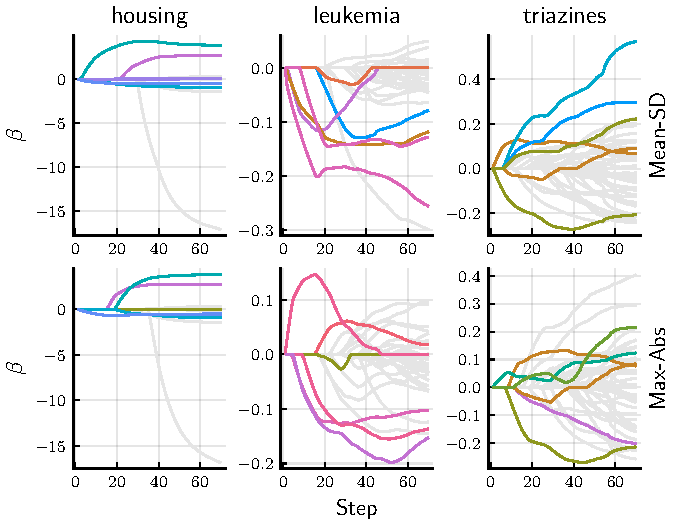
\includegraphics[]{plots/realdata_paths.pdf}
  \caption{%
    Lasso paths for real datasets using two types of normalization:
    standardization and maximum absolute value normalization (max--abs). We have fit
    the lasso path to two different datasets:
    \data{housing}~\citep{harrison1978}, \data{leukemia}~\citep{golub1999},
    \data{triazines}~\citep{king}, and \data{w1a}~\citep{platt1998}. (See \Cref{sec:data-summary}
    for more information about these data sets.) For each
    dataset, we have colored the coefficients if they were among the first five
    to become non-zero under either of the two normalization schemes. We see
    that the paths differ with regards to the size as well as the signs of the
    coefficients, and that, in addition, the features to become active first
    differ between the normalization types.
  }
  \label{fig:realdata-paths-full}
\end{figure}

\subsection{Bias and Variance of Lasso and Ridge Estimators}%
\label{sec:additional-results-biasvar}

\begin{figure}[htpb]
  \centering
  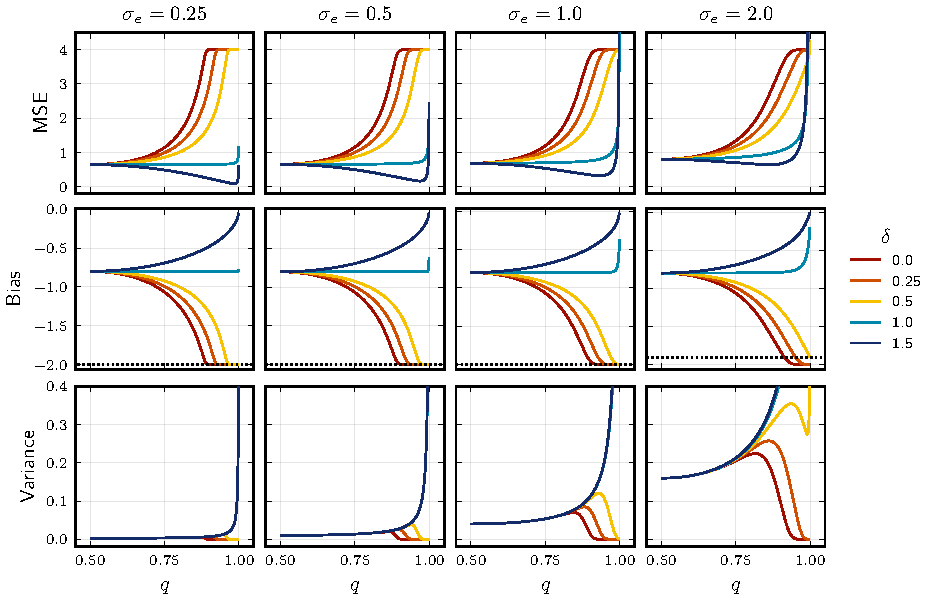
\includegraphics[]{plots/binary_onedim_bias_var_lasso.pdf}
  \caption{%
    Bias, variance, and mean-squared error for a one-dimensional lasso problem,
    parameterized by noise level (\(\sigma_\varepsilon\)), class balance (\(q\)), and
    scaling (\(\delta\)). Dotted lines represent asymptotic bias of the lasso
    estimator in the case when \(\delta = 1/2\).}
  \label{fig:bias-var-onedim-lasso-full}
\end{figure}

\begin{figure}[htpb]
  \centering
  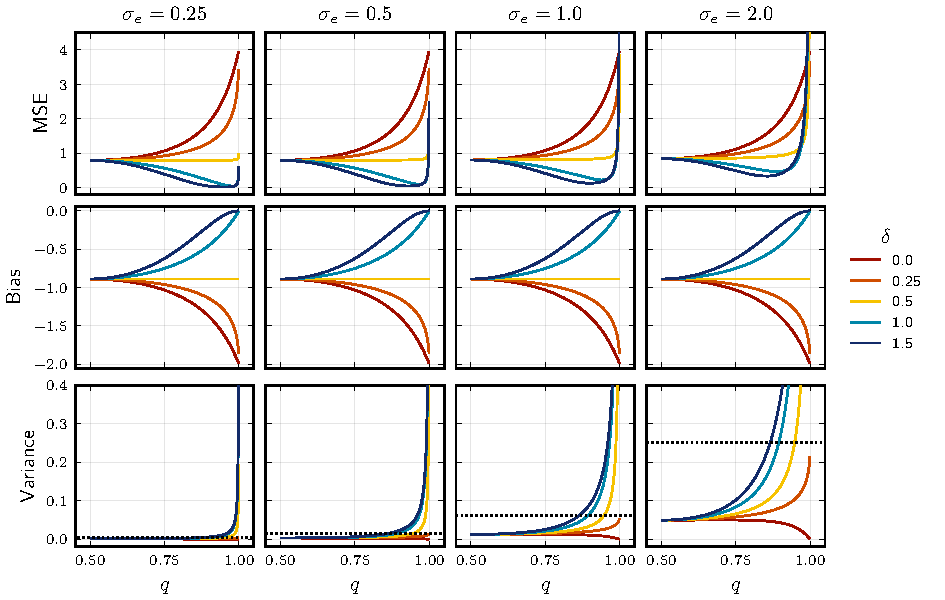
\includegraphics[]{plots/binary_onedim_bias_var_ridge.pdf}
  \caption{%
    Bias, variance, and mean-squared error for one-dimensional ridge regression,
    parameterized by noise level (\(\sigma_\varepsilon\)), class balance (\(q\)), and
    scaling (\(\delta\)). Dotted lines represent asymptotic bias of the ridge
    estimator in the case of \(\delta = 1/4\).}
  \label{fig:bias-var-onedim-ridge-full}
\end{figure}

\begin{figure}[htpb]
  \centering
  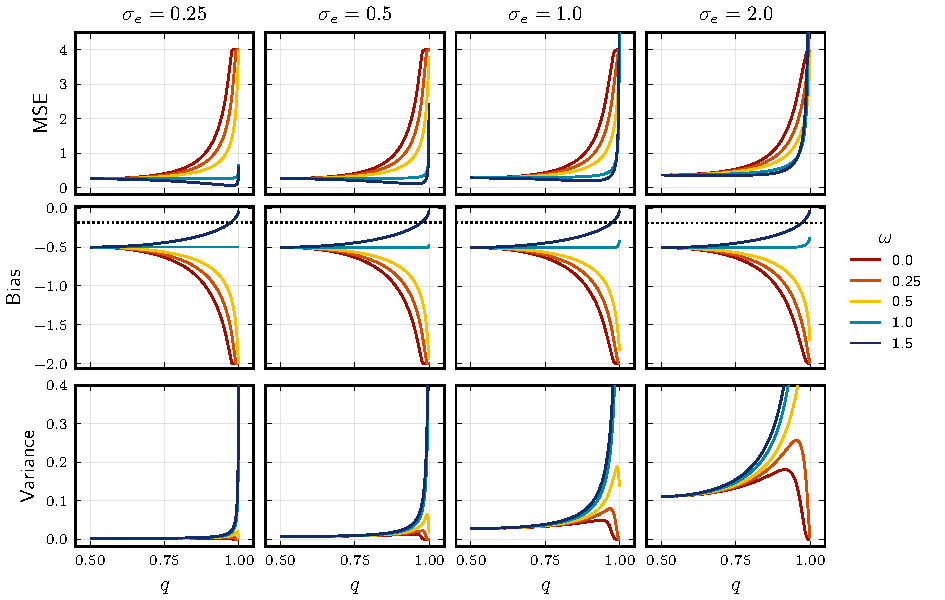
\includegraphics[]{plots/binary_onedim_bias_var_elnet.pdf}
  \caption{%
    Bias, variance, and mean-squared error in the case of the one-dimensional weighted elastic
    net. The measures are shown for different noise levels (\(\sigma_\varepsilon\)), class
    balances (\(q_j\)), and values of (\(\omega\)), which controls the weights that are set to
    \(u_j = v_j = 2\times 4^{\omega - 1}(q-q^2)^\omega\) in order for the results to be
    comparable across different values of \(\omega\). The dotted lines represent the asymptotic
    bias of the estimator in the case of \(\omega = 1\). In the case of \(\omega > 1\), the
    limit of the bias is zero.
  }
  \label{fig:binary-onedim-bias-var-elnet-full}
\end{figure}

\begin{figure}[htpb]
  \centering
  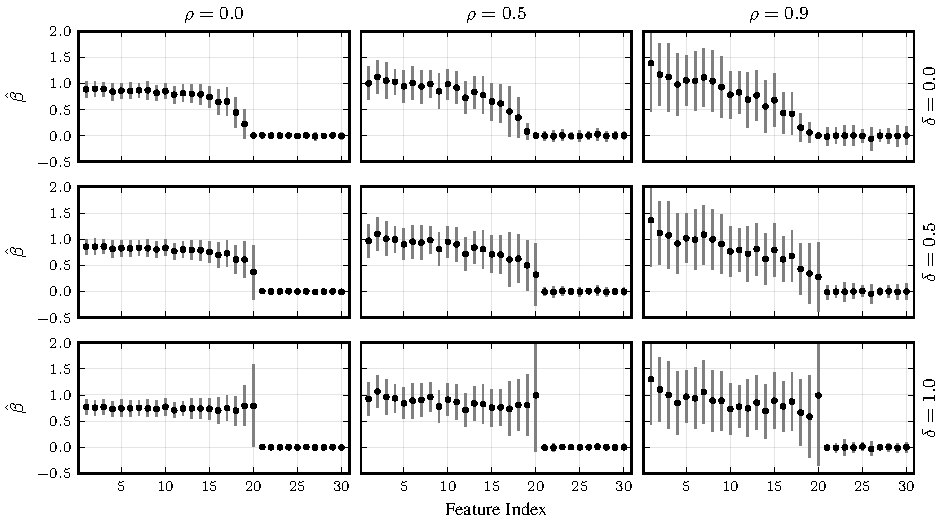
\includegraphics[]{plots/binary_decreasing.pdf}
  \caption{%
    Estimates of the regression coefficients from the lasso, \(\hat{\vec{\beta}}\), for the
    first 30 coefficients in the experiment. All of the features are binary and the first 20
    features correspond to true signals with \(\beta_j^* = 2\) and geometrically decreasing
    class balance from 0.5 to 0.99. The remaining features have class balance \(q_j \in [0.5,
      0.99]\) distributed linearly among the features. The plot shows means and standard
    deviations averaged over 50 iterations.
  }
  \label{fig:binary-decreasing-full}
\end{figure}

In \Cref{fig:hyperopt-support}, we have, in addition to NMSE on the validation set, also
plotted the size of the support of the lasso (cardinality of the set of features that have
corresponding nonzero coefficients). Here we only show results for \(\delta \in \{0, 1/2,
1\}\). It is clear that \(\delta = 1/2\) works quite well for all of these three data sets,
being able to attain a value close to the mininum for each of the three data sets. This is
not the case for \(\delta \in \{0, 1\}\), for which the best possible prediction error is
considerably worse. This is particularly the case with \(\delta =0\) and the \data{w1a}
data set. The dependency between \(\lambda\) and \(\delta\) is also visible here by looking
at the support size.

\begin{figure}[htpb]
  \centering
  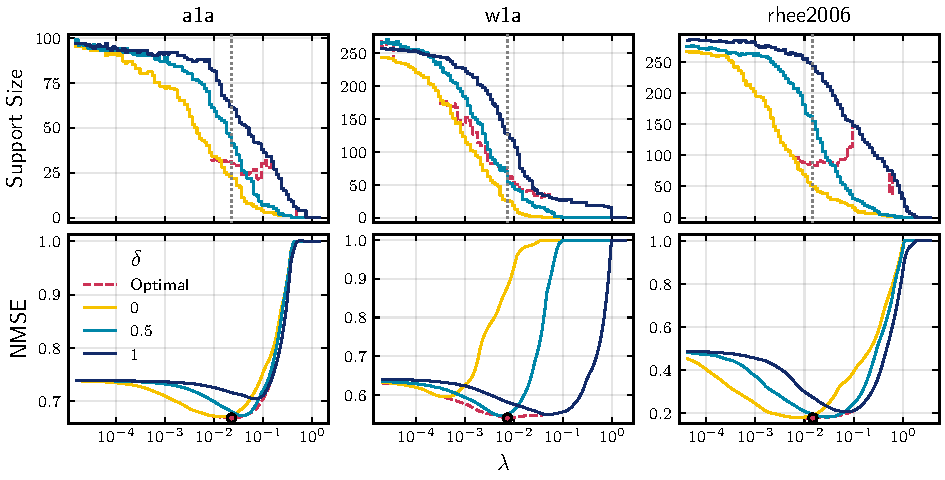
\includegraphics[]{plots/hyperopt_paths.pdf}
  \caption{%
    Support size and normalized mean-squared error (NMSE) for the validation set for the lasso
    fit to datasets \data{a1a}, \data{w1a}, and \data{rhee2006} across combinations of
    \(\delta\) and \(\lambda\). The optimal \(\delta\) is marked with dashed black lines and
    the best combination of \(\delta\) (among 0, 1/2, and 1) and \(\lambda\) is shown as a dot.
  }
  \label{fig:hyperopt-support}
\end{figure}
